\documentclass{article}

% Language setting
% Replace `english' with e.g. `spanish' to change the document language
\usepackage[english]{babel}

% Set page size and margins
% Replace `letterpaper' with `a4paper' for UK/EU standard size
\usepackage[letterpaper,top=2cm,bottom=2cm,left=3cm,right=3cm,marginparwidth=1.75cm]{geometry}
\usepackage{tikz}
\usepackage{amsfonts}
\usepackage{amssymb}

% Useful packages
\usepackage{amsmath}
\usepackage{graphicx}
\usepackage[colorlinks=true, allcolors=blue]{hyperref}

\setcounter{MaxMatrixCols}{20}


\title{Project 2024 - Markov Chains}
\author{
    \begin{center}
        Paul.G - Shreyas.V - Clayton.H - Samuel.M - Alexis.L
    \end{center}
}

\begin{document}
    \maketitle
    \section*{Five states Mediterranean ecosystems}
    \subsection*{Q1-/ Draw the graph associated to this model.}
    \begin{figure}[h]
        \centering
        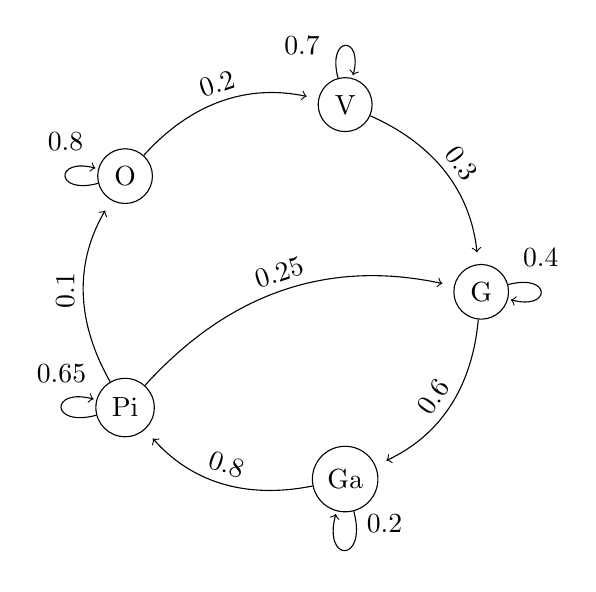
\begin{tikzpicture}
            % Set the radius for the circular arrangement of nodes
            \def\radius{2.5}

            % Draw the nodes in a circular arrangement

            \node[circle, draw] (V) at ({1 * 72}:\radius) {V};
            \node[circle, draw] (O) at ({2 * 72}:\radius) {O};
            \node[circle, draw] (Pi) at ({3 * 72}:\radius) {Pi};
            \node[circle, draw] (Ga) at ({4 * 72}:\radius) {Ga};
            \node[circle, draw] (G) at ({5 * 72}:\radius) {G};

            \path[->, shorten >=1.5mm] (O) edge [bend left] node[midway, sloped, above] {$0.2$} (V);
            \path[->, shorten >=1.5mm] (V) edge [loop above] node [left=0.2cm]  {$0.7$} (V);

            \path[->, shorten >=1.5mm] (Pi) edge [bend left] node[midway, sloped, above] {$0.1$} (O);
            \path[->, shorten >=1.5mm] (O) edge [loop left] node [above=0.2cm]  {$0.8$} (O);

            \path[->, shorten >=1.5mm] (Ga) edge [bend left] node[midway, sloped, above] {$0.8$} (Pi);
            \path[->, shorten >=1.5mm] (Pi) edge [loop left] node [above=0.2cm]  {$0.65$} (Pi);

            \path[->, shorten >=1.5mm] (G) edge [bend left] node[midway, sloped, above] {$0.6$} (Ga);
            \path[->, shorten >=1.5mm] (Ga) edge [loop below] node [right=0.5cm, above=0.1cm]  {$0.2$} (Ga);

            \path[->, shorten >=1.5mm] (V) edge [bend left] node[midway, sloped, above] {$0.3$} (G);
            \path[->, shorten >=1.5mm] (G) edge [loop right] node [above=0.2cm]  {$0.4$} (G);

            \path[->, shorten >=1.5mm] (Pi) edge [bend left] node[midway, sloped, above] {$0.25$} (G);
            % Draw edges between each pair of outer nodes
        \end{tikzpicture}
    \end{figure}

    \subsection*{Q2-/ Supposing that we are in state Pi, what is the probability of a trajectory of the type Pi-G-Ga? And of a trajectory of the type Pi-O-V?}

    Since we have a weighted graph,
    \begin{itemize}
        \item $\text{P}(Pi-G-Ga) = \text{P}(Pi \cap G \cap Ga|Pi) = \text{P}(Pi|Pi)*\text{P}(G|Pi)*\text{P}(Ga|G)$
        $= 0.65*0.25*0.6 = 0.0975$
        \item $\text{P}(Pi-O-V) = \text{P}(Pi \cap O \cap V|Pi) = \text{P}(Pi|Pi)*\text{P}(O|Pi)*\text{P}(V|O)$
        $= 0.65*0.1*0.2 = 0.013$
    \end{itemize}



    \subsection*{Q3-/ Give an example of a trajectory with a vanishing probability}

    We can take any trajectory for witch we have a zero probability to go from a vertex to another in the transition probability matrix.\\[1em]
    For example we see that the trajectory from garrigue (Ga) to oakgrove (O) has a vanishing probability

    \subsection*{Q4-/ Using a computer,compute the distribution of the ecosystem for n=20}

    X\(_0\) is a uniform distribution, then all possible values of X are equally likely so we have \( X_0 = \begin{bmatrix} 0.2 \\ 0.2 \\ 0.2 \\ 0.2 \\ 0.2 \end{bmatrix} \).\\[1em]
    Then we multiply  n=20 times the transition probability matrix by P X\(_0\)  . We can use a for loop to do P*X\(_0\) 20 times or directly do \( P^{20} * X_0 \) witch gives \( X_{20} = \begin{bmatrix} 0.1752 \\ 0.1166 \\ 0.2044 \\ 0.1533 \\ 0.3505 \end{bmatrix} \).

    \subsection*{Q5-/ Plot the evolution of the ecosystem’s distribution as a function of n}

    \begin{figure}[h]
        \centering
        \includegraphics[width=0.7\linewidth]{ecosystem_distribution}
        \caption{\label{fig:evo}Evolution of the ecosystem’s distribution as a function of $n$}
    \end{figure}
    We can see that:
    \begin{itemize}
        \item Over time, each population seems to approach a stable equilibrium, a limit.
        \item The Pine forest (Pi) population grows significantly more than the other populations.
        \item The Grass (G) population decreases slightly before returning to its initial state.
        \item Garrigue (Ga), oakgrove (O) and Vineyards and orchards (V) populations are decreasing.
    \end{itemize}

    \subsection*{Q6-/ Using your Linear Algebra course (and MATLAB for the computations), diagonalize \( P \). In other words, find matrices \( A \), \( A^{-1} \), and \( D \) (with \( D \) diagonal) such that \( P = A D A^{-1} \). What do the matrices \( A \), \( A^{-1} \), and \( D \) represent in terms of eigenvalues and eigenstates?}


    \section*{A more complex model for a more diverse ecosystem}

    \subsection*{Q9-/ Give the groups of states that all communicate with each other.
    Explain how this can be seen on the matrix.}
    Here the groups of states that all communicate with each other :
    \section*{Communicating State Pairs}
    \begin{center}

        \begin{tabular}{|c|c|c|}
            \hline
            1 - 3  & 1 - 5  & 2 - 3  \\ \hline
            3 - 4  & 3 - 5  & 9 - 10 \\ \hline
            9 - 11 & 10 - 11 & 13 - 14 \\ \hline
            13 - 15 & 13 - 16 & 13 - 17 \\ \hline
            13 - 18 & 14 - 15 & 14 - 16 \\ \hline
            14 - 17 & 14 - 18 & 14 - 19 \\ \hline
            14 - 20 & 15 - 16 & 15 - 17 \\ \hline
            15 - 19 & 15 - 20 & 16 - 17 \\ \hline
            16 - 18 & 16 - 19 & 16 - 20 \\ \hline
            17 - 18 & 17 - 19 & 17 - 20 \\ \hline
            18 - 19 & 18 - 20 & 19 - 20 \\ \hline
        \end{tabular}
    \end{center}

    \section*{Steps to verify communications :}
    \begin{itemize}
        \item Let i for rows and j for columns
        \item We have to avoid all the redundant values like (i,j) if (j,i) is already considered.
        \item We have to see if there exists a direct or indirect transition from state (i to j) or (j to i)

    \end{itemize}


    \subsection*{Q10-/ Start from the distribution \( X_0 \)}
    \subsection*{(a) Compute the distribution \( X_n \) of the system for \( n = 2\), \(n = 10\) and \(n = 50 \)}
    We will use the transition formula:
    \[
        X_n = P^n X_0,
    \]
    where \( P \) is the given transition matrix.
    \item For \(n = 2\),
    \[
        X_2 = \begin{pmatrix}
                  0.11 & 0.105 & 0.515 & 0.12 & 0.15 & 0 & 0 & 0 & 0 & 0 & 0 & 0 & 0 & 0 & 0 & 0 & 0 & 0 & 0 & 0
        \end{pmatrix}^T,
    \]
    \item For \(n = 10\),
    \[
        X_{20} = \begin{pmatrix}
                     0.26 & 0.1064 & 0.2363 & 0.1717 & 0.2256 & 0 & 0 & 0 & 0 & 0 & 0 & 0 & 0 & 0 & 0 & 0 & 0 & 0 & 0 & 0
        \end{pmatrix}^T,
    \]
    \item For \(n = 50\),
    \[
        X_{50} = \begin{pmatrix}
                     0.2601 & 0.1064 & 0.2362 & 0.1717 & 0.2256 & 0 & 0 & 0 & 0 & 0 & 0 & 0 & 0 & 0 & 0 & 0 & 0 & 0 & 0 & 0
        \end{pmatrix}^T,
    \]


    \subsection*{(b) Plot \( X_n \) as a function of \( n \)}

    \includegraphics[width=\textwidth]{graph_Xn.png}

    \subsection*{(c) Does th sequence \( (X_n)_{n \in \mathbb{N}} \) admit a limiting distribution ?}
    By looking at the graph, we can see that the sequence seems to admit a limiting distribution. To be sure let's take n = 999 and lets compare \( X_{1000}\) with \( X_{50} \):
    \[
        X_{50} = \begin{pmatrix}
                     0.2601 & 0.1064 & 0.2362 & 0.1717 & 0.2256 & 0 & 0 & 0 & 0 & 0 & 0 & 0 & 0 & 0 & 0 & 0 & 0 & 0 & 0 & 0
        \end{pmatrix}^T,
    \]

    \[
        X_{999} = \begin{pmatrix}
                      0.2601 & 0.1064 & 0.2362 & 0.1717 & 0.2256 & 0 & 0 & 0 & 0 & 0 & 0 & 0 & 0 & 0 & 0 & 0 & 0 & 0 & 0 & 0
        \end{pmatrix}^T,
    \]

    We clearly see that the value remain the same. Hence, the sequence \( (X_n)_{n \in \mathbb{N}} \) admit a limiting distribution.

    \subsection*{Q11-/ Now start from the distribution \( Y_0 \)}
    \subsection*{(a) Compute the distribution \( Y_n \) of the system for \( n = 2\), \(n = 10\) and \(n = 50 \)}
    Simmilarly, we will use the transition formula:
    \[
        Y_n = P^n Y_0,
    \]
    where \( P \) is the given transition matrix.
    \item For \(n = 2\),
    \[
        Y_2 = \begin{pmatrix}
                  0 & 0 & 0 & 0 & 0 & 0 & 1 & 0 & 0 & 0 & 0 & 0 & 0 & 0 & 0 & 0 & 0 & 0 & 0 & 0
        \end{pmatrix}^T,
    \]
    \item For \(n = 10\),
    \[
        Y_{20} = \begin{pmatrix}
                     0 & 0 & 0 & 0 & 0 & 0 & 1 & 0 & 0 & 0 & 0 & 0 & 0 & 0 & 0 & 0 & 0 & 0 & 0 & 0
        \end{pmatrix}^T,
    \]
    \item For \(n = 50\),
    \[
        Y_{50} = \begin{pmatrix}
                     0 & 0 & 0 & 0 & 0 & 0 & 1 & 0 & 0 & 0 & 0 & 0 & 0 & 0 & 0 & 0 & 0 & 0 & 0 & 0
        \end{pmatrix}^T,
    \]


    \subsection*{(b) Plot \( Y_n \) as a function of \( n \)}

    \includegraphics[width=\textwidth]{graph_Yn.png}

    \subsection*{(c) Does th sequence \( (Y_n)_{n \in \mathbb{N}} \) admit a limiting distribution ?}
    By looking at the graph, we can see that the sequence does not admit a limiting distribution. To be sure let's take n = 999 and lets compare \( X_{1000}\) with \( X_{50} \):
    \[
        Y_{50} = \begin{pmatrix}
                     0 & 0 & 0 & 0 & 0 & 0 & 1 & 0 & 0 & 0 & 0 & 0 & 0 & 0 & 0 & 0 & 0 & 0 & 0 & 0
        \end{pmatrix}^T,
    \]

    \[
        Y_{999} = \begin{pmatrix}
                      0 & 0 & 0 & 0 & 0 & 0 & 0 & 1 & 0 & 0 & 0 & 0 & 0 & 0 & 0 & 0 & 0 & 0 & 0 & 0
        \end{pmatrix}^T,
    \]

    We clearly see that the value does not remain the same, in fact it switches between the 7th row and the 8th row. Hence, the sequence \( (Y_n)_{n \in \mathbb{N}} \) is unstable at +infinity so it doesn't admit a limiting distribution.

    \subsection*{Q12-/ Same questions strating from the initial distributions \( Z_0 \) and \( W_0 \)}
    \subsection*{(a) Compute the distribution \( Y_n \) of the system for \( n = 2\), \(n = 10\) and \(n = 50 \)}
    Simmilarly, we will use the transition formula:
    \[
        Y_n = P^n Y_0,
    \]
    where \( P \) is the given transition matrix.
    \section*{Question 12}

    For \( Z_n \):
    \[
        \begin{aligned}
            &n = 2: \ Z_2 = [0, 0, 0, 0, 0, 0, 0, 0.6, 0.1, 0.03, 0.03, 0, 0, 0, 0, 0, 0, 0, 0, 0]^{T} \\
            &n = 10: \ Z_{10} = [0.0432, 0.0167, 0.0388, 0.0282, 0.0412, 2.43 \times 10^{-4}, 7.29 \times 10^{-5}, 2.187 \times 10^{-5}, \\
            &\quad \quad 6.561 \times 10^{-6}, 1.9683 \times 10^{-6}, 0, 0, 0, 0, 0, 0, 0, 0, 0]^{T} \\
            &n = 50: \ Z_{50} = [0.484, 0.0197, 0.0442, 0.0324, 0.0417, 2.954 \times 10^{-25}, 8.8629 \times 10^{-26}, \\
            &\quad \quad 2.6589 \times 10^{-26}, 7.9766 \times 10^{-27}, 2.393 \times 10^{-27}, 2.393 \times 10^{-27}, 0, 0, 0, 0, 0, 0, 0, 0, 0]^{T}
        \end{aligned}
    \]

    For \( W_n \):
    \[
        \begin{aligned}
            &n = 2: \ W_2 = [0, 0, 0, 0, 0, 0, 0, 0, 0, 0, 0, 0, 0.53, 0.155, 0.1, 0.105, 0.085, 0.145, 0.04, 0.0825]^{T} \\
            &n = 10: \ W_{10} = [0, 0, 0, 0, 0, 0, 0, 0, 0, 0, 0, 0, 1.0525, 0.0101, 0.0056, 0.0056, 0.0053, 0.0075, 0.0024, 0.0025]^{T} \\
            &n = 50: \ W_{50} =[0, 0, 0, 0, 0, 0, 0, 0, 0, 0, 0, 0, 1.0817, 4.4996 \times 10^{-9}, 2.5013 \times 10^{-9}, 2.4982 \times 10^{-9}, \\
            &\quad \quad 2.3432 \times 10^{-9}, 3.3164 \times 10^{-9}, 1.0574 \times 10^{-9}, 1.1181 \times 10^{-9}]^{T}
        \end{aligned}
    \]

    \section*{Question 13}
    \subsection*{(a)  Compute of \( \alpha_n \) distribution }
    For \( \alpha_n \):
    \[
        \begin{aligned}
            &n = 2: \ \alpha_2 = [0, 0, 0, 0, 0.2, 0, 1, 0, 0, 0, 0, 0, 0, 0, 0, 0, 0, 0, 0, 0]^{T} \\
            &n = 10: \ \alpha_{10} = [0.0589, 0.0235, 0.0528, 0.0392, 0.0531, 0, 0, 0, 0, 0, 0, 0, 0, 0, 0, 0, 0, 0, 0, 0]^{T}\\
            &n = 50: \ \alpha_{50} = [0.0654, 0.0267, 0.0597, 0.0437, 0.0563, 0, 0, 0, 0, 0, 0, 0, 0, 0, 0, 0, 0, 0, 0, 0]^{T}
        \end{aligned}
    \]
    \subsection*{(b) Plot of \( \alpha_n \) as a function of \( n \)}
    \begin{figure}[h]
        \centering
        \includegraphics[width=0.7\linewidth]{plot_alpha_n.png}
        \caption{\label{fig:evo} $\alpha$ as a function of $n$}
    \end{figure}
    \subsection*{(c) Linear relation between the limiting distributions of $(\alpha_n)_{n \in \mathbb{N}}$, $(X_n)_{n \in \mathbb{N}}$, and $(W_n)_{n \in \mathbb{N}}$}


\end{document}
































































